\documentclass[11pt]{article} % For LaTeX2e
\usepackage{rldm,palatino}
\usepackage{graphicx}
\usepackage{multicol}
\usepackage{amsmath}
\usepackage{amsfonts}

\usepackage[colorlinks,urlcolor=blue,bookmarks=false,hypertexnames=true]{hyperref}

% Beautiful Biblatex!
\usepackage[%
backend=biber,%
style=authoryear-comp,%
backref=false,%
sortcites=true,sorting=nyt,%
mincitenames=1,maxcitenames=2%
]{biblatex}

\addbibresource{paper.bib}

\title{Predictions Predicting Predictions} % which Predict Predictions}

\setlength\bibitemsep{0.7\itemsep}

\author{
  Matthew K. Schlegel\thanks{mkschleg.github.io} \\
  Department of Computing Science \\
  University of Alberta\\
  \texttt{mkschleg@ualberta.ca} \\
  \And
  Martha White \\
  Department of Computing Science \\
  University of Alberta \\
  \texttt{whitem@ualberta.ca}
}

% The \author macro works with any number of authors. There are two commands
% used to separate the names and addresses of multiple authors: \And and \AND.
%
% Using \And between authors leaves it to \LaTeX{} to determine where to break
% the lines. Using \AND forces a linebreak at that point. So, if \LaTeX{}
% puts 3 of 4 authors names on the first line, and the last on the second
% line, try using \AND instead of \And before the third author name.

\newcommand{\fix}{\marginpar{FIX}}
\newcommand{\new}{\marginpar{NEW}}

\newcommand{\citeplease}{\textbf{[CITE]}}
\newcommand{\refplease}{\textbf{[REF]}}

\begin{document}

\maketitle

\begin{abstract}
  Predicting the sensorimotor stream has consistently been a key component for building general learning agents. Whether through predicting a reward signal to select the best action or learning a predictive world model with auxiliary tasks, prediction making is at the core of reinforcement learning. One of the main research directions in predictive architectures is in the automatic construction of learning objectives and targets. The agent can consider any real-valued signal as a target when deciding what to learn, including the current set of internal predictions. A prediction whose learning target is another prediction is known as a composition. Arbitrarily deep compositions can lead to learning objectives that are unstable or not suitable for function approximators. This manuscript looks to begin uncovering the underlying structure of compositions in an effort to leverage and learn them more effectively in general learning agents. Specifically, we consider the dynamics of compositions both empirically and analytically. We derive the effective schedule of emphasis (or discounts) of future observations with compositions of arbitrary depth, leading to informative observations about the prediction targets. In the empirical simulations, we focus on the unintuitive behavior of compositions, especially in cases that are not easy to analyze. Overall, predictions predicting predictions which predict predictions have interesting properties and can add depth to an agent's predictive understanding of the world.
  
  % Predicting the sensori-motor stream has consistently been a key
  % component for building general learning agents. Whether through
  % predicting a reward signal to select the best action or learning
  % a predictive world model with auxiliary tasks,
  % prediction making are at the core of
  % reinforcement learning.
  % In these architectures, we not only want the agent to leverage predictions
  % for better control but also to have the agent decide what
  % learning objectives and targets to consider. The agent can consider
  % any real-valued signal as a target, including the set of predictions the agent
  % is already making. This enables the agent to predict predictions, which can
  % lead to arbitrarily deep compositions of predictions.
  % We consider the dynamics of these compositions both
  % empirically and analytically. The analytical form provides a new set
  % of discount schedules, giving insight into how samples are
  % emphasized in compositions. The empirical simulations
  % focus on the sometimes unintuitive behaviour of compositions. We also
  % pose several future directions and questions spurred by these
  % observations.

  % focusing on the effective discount
  % function and returns from simulations. Specifically, we derive the
  % analytical form of the effective discount function for $n$
  % compositions of a constant discount, provide empirical observations
  % of more interesting compositions, and discuss future directions and
  % questions to further understand predictions which predict other predictions.

  % The intuition that an agent should
  % learn about its environment through span independent predictions is
  % pleasing.
  % \begin{itemize}
  % \item GVFs + Predicting the world w/ span independent predictions
  % \item Automatic Discovery, compositions
  % \item What is the effect of compositions.
  % \item Construct the associated discounting sequence for compositions
  %   in a general form.
  % \item Analyze the sequences
  % \item Provide some empirical simulations of more complex discounting schemes.
  % \end{itemize}
  
  % Within the GVF framework, an agent can make deci
  
% The \emph{title} should be a maximum of 100 characters. 

% The \emph{abstract} should be a maximum of 2000 characters of text,
% including spaces (no figure is allowed). You will be asked to copy
% this into a text-only box; and it will appear as such in the
% conference booklet. Use 11~point type, with a vertical spacing of
% 12~points.  The word \textbf{Abstract} must be centered, bold, and in
% point size 12. Two line spaces precede the abstract.
\end{abstract}

\keywords{reinforcement learning; prediction; GVFs}

\acknowledgements{We would like to thank the Alberta Machine
  Intelligence Institute, IVADO, NSERC and the Canada CIFAR AI Chairs
  Program for the funding for this research. We would also like to
  thank Andrew Patterson for his insightful comments about the
  connection to digital signal processing and Adam White for
  sharing the Critterbot dataset.}


\startmain % to start the main 1-4 pages of the submission.

\section{Introduction}

% Recently, there has been interest in using temporal-difference
% learning to learn value functions of arbitrary sensori-motor signals
% accessible by the agent \cite{sutton2011, modayil2014} \citeplease.
% These value functions are known as general value functions (GVFs), and
% are a convenient set of semantics for posing predictive questions
% \cite{white2015}.

% The horde architecture and GVFs have been applied to
% several interesting problems in reinforcement learning. Possibly the
% widest used is through auxiliary tasks \citeplase. Auxiliary tasks are
% unsupervised predictions of the data stream which are hypothesized to
% improve the signal to learn better representations. They have been
% successful empirically, with many variants including automatic
% discovery of questions \citeplease. Another application of GVFs is
% as the semantics for predictive questions in a predictive
% representation \citeplease. GVFs have also been used to build a
% model... thesis please....

Reinforcement learning is built on predicting the effect of behavior
on future observations and rewards. Many of our algorithms learn
predictions of a cumulative sum of (discounted) future rewards, which
is used as a bedrock for learning desirable policies. While reward has
been the primary predictive target of focus, TD models
\parencite{sutton1995td} lay out the use of temporal-difference
learning to learn a world model through value function
predictions. Temporal-difference networks
\parencite{sutton2004temporal} take advantage of this abstraction and
build state and representations through
predictions. \cite{sutton2011} and
\cite{white2015} further the predictive
perspective by developing a predictive approach to building world
knowledge through general value functions (GVFs).

GVFs have been pursued broadly in reinforcement learning: \cite{gunther2016intelligent} used GVFs to build an open loop laser welder controller, \cite{linke2020adapting} used predictions and their learning progress to develop an intrinsic reward, \cite{edwards2016application} used GVFs to build controllers for myoelectric prosthetics, using gvfs for auxiliary training tasks to improve representation learning \parencite{jaderberg2017,veeriah2019discovery}, to extend a value function's approximation to generalize over goals as well as states \parencite{schaul2015universal}, and to create a scheduled controller from a set of sub-tasks for sparse reward problems \parencite{riedmiller2018learning}. Successor
representations and features are predictions of the state, learned or
given, which have been shown to improve learning performance
\parencite{dayan1993, russek2017, barreto2018, sherstan2018}.

Learning predictions of any real-valued signal the agent has access to
also opens the possibility of asking compositional predictive
questions \parencite{white2015}. A compositional question is one whose
target is dependent on another prediction internal to the
agent. Compositions expand the possible range of predictive questions
we can specify as a GVF  \parencite{sutton2004temporal,
  rafols2006, white2015, schlegel2021general,
  zheng2021learning}. While this may suggest the GVF framework is
limited in what questions can be asked, the limitations are necessary
so the predictions can be trained \emph{independent of
span} \parencite{van2015learning}. Learning independent of span means the
target can be learned using online algorithms regardless of the effective horizon
of the prediction. Adding layers of compositional questions have
improved the learning in predictive representations
\parencite{rafols2006, schlegel2021general}, and improved the performance
of deep reinforcement learning through auxiliary tasks
\parencite{zheng2021learning}. In the automatic specification of
learning targets compositions are thought to provide a way for the agent
to build complexity \parencite{schlegel2021general, veeriah2019discovery,
kearney2022, zheng2021learning}, but often these architectures don't
leverage compositions for stability concerns
\parencite{schlegel2021general}. 


As well as improving behavior empirically, compositions can provide
semantic depth. An excellent example of this can be seen in
option-extended temporal difference networks \parencite{rafols2006},
and later explored again in \cite{schlegel2021general}.
The example is centered in an environment where the agent has a
low-powered visual sensor and needs to learn its directionality from
the painted walls. Each cardinal
direction has a different colored wall. The first layer of predictions
the agent makes is to predict what color it will observe if it were to
drive straight. The second layer are myopic predictions
which ask what the first layer's prediction will be after turning
clockwise (or counter-clockwise). The second layer allows the agent to
predict which walls are to its sides as well as the wall in the
direction the agent is facing.
These predictions cannot be specified in the usual GVF framework,
but can be easily constructed through compositions.
While this may be ``repeated information'' in a sense, the extra
learning objectives makes the learning properties of the predictive
representation better as compared to other specifications \parencite{schlegel2021general}.

As algorithms for the automatic discovery of complex question networks
continue to push the boundaries of what questions are considered by
the agent, the properties of compositions should be better studied.
When searching for what to learn the questions an agent eventually
retains will be dependent on the agent's ability to learn the
predictions.
While it is clear
questions that naturally diverge (say setting the discount
$\gamma=1$) should be avoided, other problems, such
as the scale of a target, could be equally as problematic when using
function approximation (i.e. end-to-end neural networks). This
could mean important predictions are disregarded because the agent is
unable to learn the answer without proper strategies to normalize the
prediction's magnitude. Better strategies for learning and normalizing
predictive targets will come from understanding the effective discount
schedule (or emphasis) compositional predictions will have on the
targets.

In this report, we consider the effect of compositions on the sequence
of discounts, and relegate the effect of off-policy importance weights
to future work.
We first analyze the sequence of discounts over any
number of compositions and constant discounts. We then analyze
this sequence to better
understand how it emphasizes parts of the data stream.
Surprisingly, the effective discount for constant discount compositions
have a form which can be described analytically. While this does
not include the full spectrum of discount functions, it provides a
first step towards understanding compositions.
Next we look at simulations using more complex state-dependent
discount functions using a simple consistent sequence and two
timeseries datasets. In these simulations we focus on the effect of
applying the same discount function a large number of times, looking
to see if the shape of the returns become regular over the
compositions. Finally, several future directions and questions are posed.
%
%
\begin{figure}
  \centering
  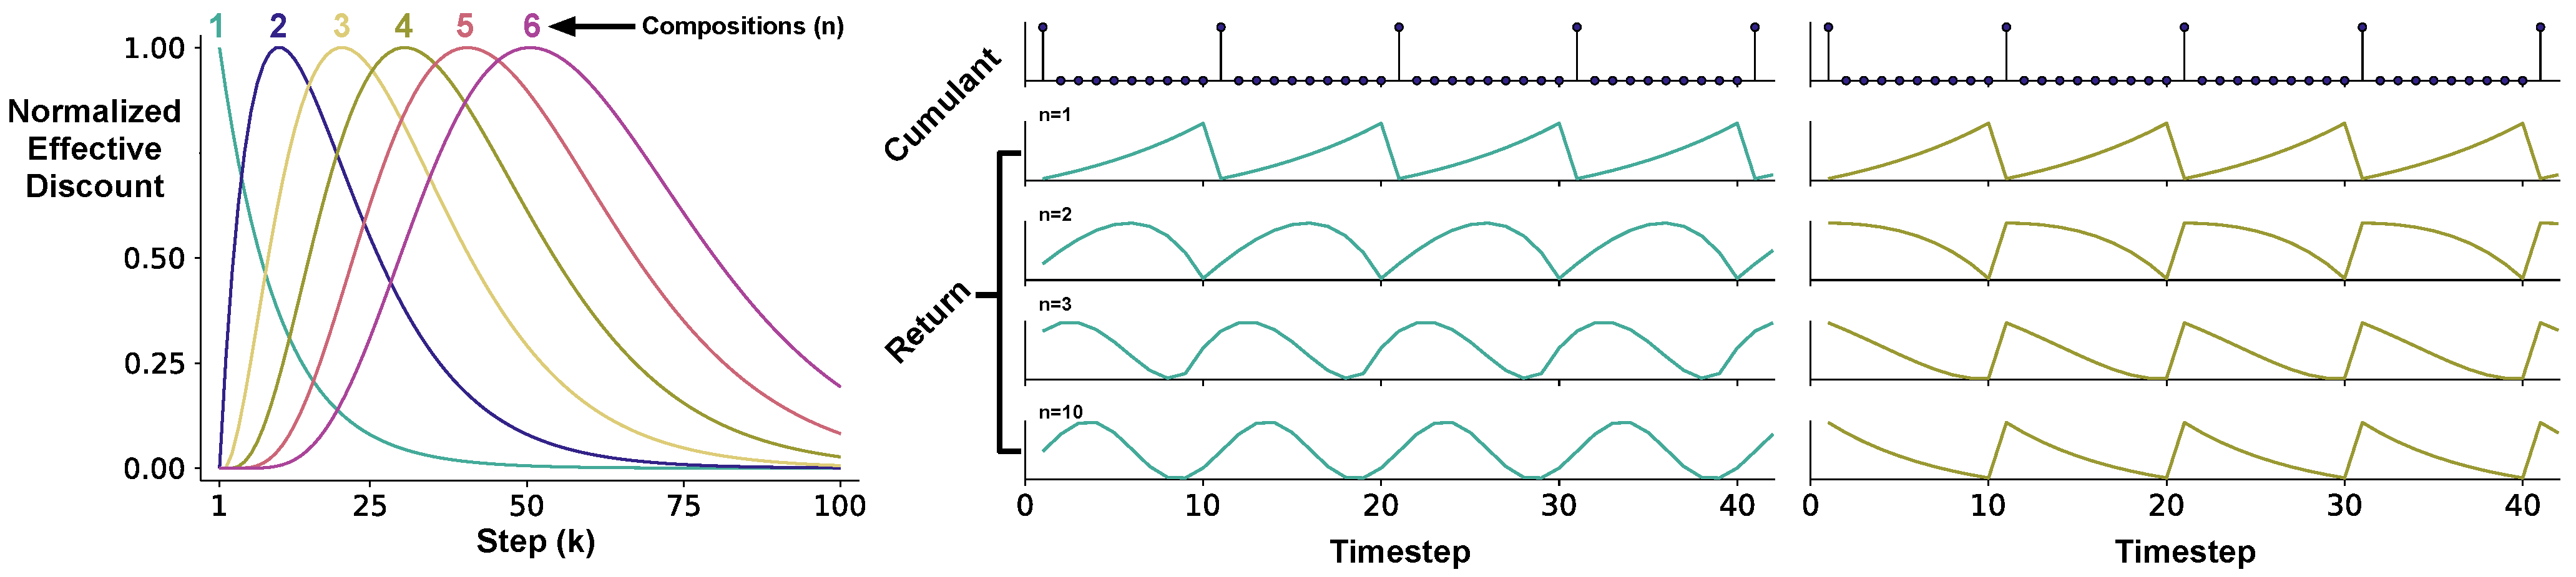
\includegraphics[width=\textwidth]{plots/seq_plus_cw.pdf}
  \caption{(\textbf{left}) The effective discount for $n$ compositions
    normalized by the maximum value found in section
    \ref{sec:analyze}. (\textbf{middle, right}) The cycle world
    simulations, with top graph as the cumulant and subsequent plots
    $n$ compositions with constant and terminating discounts
    respectively. \vspace{-0.3cm}} \label{fig:seq_cw}
\end{figure}
%
%
\section{Analyzing the sequence}\label{sec:analyze}

In this section, we restrict to the setting where we have an infinite sequence of
sensor readings $\mathbf{x} = \{x[0], x[1], \ldots,
x[t], \ldots, x[\infty]\}$ where $x[i] \in
[x_{\text{min}} , x_{\text{max}}]$ and a constant discount $\gamma$.
The return of this signal starting at a time step $t$ is
%
$V[t] = \sum_{k=0}^\infty x[k] \gamma[k-t]$
%
%
where $\gamma[k] = \gamma^{k-1}$ for $k >= 1$ and $0$ otherwise. This
framing of the return is slightly different from the typical
presentation. Specifically, we reinterpret the return as a convolution
beteween $\gamma$ and $x$ \footnote{In digital signal processing
  \parencite{oppenheim2010discrete} often the
  convolution, in this
  case $\gamma$, is mirrored across $t$ and the inifinte sequence of
  sensor readings is $\mathbf{x} = \{x[-\infty], \ldots,
x[t], \ldots, x[\infty]\}$. The corresponding convolution
  would be $V[t] = \sum_{k=-\infty}^\infty x[k] \gamma[t-k]$ which
  would change how we define the sequence of $\gamma$. To be
  consistent with the reinforcement learning literature, we don't
  follow this here and instead implicitly define $\gamma$ as the
  mirrored version and only consider the sequence starting at $k=0$.}
and shift the discount sequence over the sensor readings.
This implicitly defines an infinite sequence
of predictions $V[t]$. In the above equation, if we replace the
sequence $x$ with the sequence of predictions $V$, we get a new set of
predictions and for any number of compositions $n$ we have
%
$V^n[t] = \sum_{k=0}^\infty V^{n-1}[k] \gamma[k-t]$.
%
Expanding this equation we can
define the general sequence of effective discounts for $n$
compositions and the corresponding return as
%
%
\[
  \gamma^n[k] = \begin{cases}
    0 \quad \mbox{ if } k < n \\
    \frac{\prod_{i=1}^{n-1} (k-i)}{(n-1)!} \gamma^{k - n}
  \end{cases} \quad\quad V^n[t] = \sum_{k=0}^\infty x[k] \gamma^n[k - t]
\]
%
where $\gamma^1[k] = \gamma[k]$ defined above and $V^n[t]$ is the
target of the $n$th composition at timestep $t$. For any value $n$ there
are two sequences multiplied together. The original discounting
shifted by the number of applications $\gamma^1[k-n]$ and a diverging
series
%
\[
  Q^n[k] = \frac{\prod_{i=1}^{n-1} (k-i)}{(n-1)!} = \frac{\Gamma(k)}{\Gamma(k-n+1)\Gamma(n)}
\]
%
where $\Gamma(k) = (k-1)!$ for $k \in \mathbb{Z}$ is known as the
Gamma function, and can be used to analyze the function with $k \in \mathbb{R}$.

We know for
any particular application of the convolution $\gamma$ on a series
with known domain $[x_{\text{min}} , x_{\text{max}}]$ the value function can take values
bounded by $V^1[t] \in [\frac{x_{\text{min}}}{1-\gamma},
\frac{x_{\text{max}}}{1-\gamma}]$. This extends to $n$ compositions in a
straightforward way where the range of the value function becomes
$V^n[t] \in [\frac{x_{\text{min}}}{(1-\gamma)^n},
\frac{x_{\text{max}}}{(1-\gamma)^n}]$.
%
% This tells us for any finite values of
% $n$ the convolution will converge, and we know it will be bounded by
% $\frac{x_{\max}}{(1-\gamma)^n}$.
%
While normalizing the value function to take values within in the
range $[0,1]$ has been used in various settings
\parencite{schlegel2021general}, as we add
more compositions we see the effective range of values shrinking
considerably.

Given the effective discounting sequence above, we can begin to piece together
the which observations are emphasized in the predictions.
The first 100 steps of the effective discount function
for several values of $n$ can be seen in figure
\ref{fig:seq_cw}.
These sequences are normalized to be in the range $[0,1]$ for a visual
comparison. The emphasis becomes increasingly spread as $n$ increases,
with the peak of this function moving further to the future at a
consistent rate.

To find the maximum value we
take the derivative of the log of the sequence with respect to $k$
getting
%
\[\frac{\delta}{\delta k} \ln \gamma^n[k] = \psi(k) - \psi(k-n+1) + \ln\gamma\]
%
where $\psi(z+1) = H_{z} - C$ is the digamma function, $H_{z} =
\sum_{i=1}^z \frac{1}{i} \leq \int_{1}^z \frac{1}{x} dx = ln(z)$ is the Euler
harmonic number, and $C$ is the Euler-Mascheroni
constant. Using the approximation above, we can find where we should
expect the maximal value is (to an approximation) $k = hn - (h-1)=h(n-1)+1$,
where $h=\frac{1}{1-\gamma}$ is sometimes known as the horizon of
discount $\gamma$. Of course this is an approximation from above and
the real value falls in $k \in [h(n-1), h(n-1) + 1)]$.


\section{Empirical observations}

While we can describe the effective discount for composing constant
discount predictions, the same techniques are difficult to apply to a
non time-invariant discount (i.e. state-dependent discounts
\parencite{white2015, sutton2011}).
Instead, in this section we look at the
ideal returns of various signals using constant discounting and a
terminating discounting functions. We use three
datasets moving from highly synthetic to real-world robot
sensori-motor data. The goal of this section is to show the
non-intuitive behavior of compositions to motivate further
analysis and exploration. All code can be found at \url{https://github.com/mkschleg/CompGVFs.jl}. Below $\gamma = 0.9$ unless otherwise stated.
%
%
\begin{figure}
  \centering
  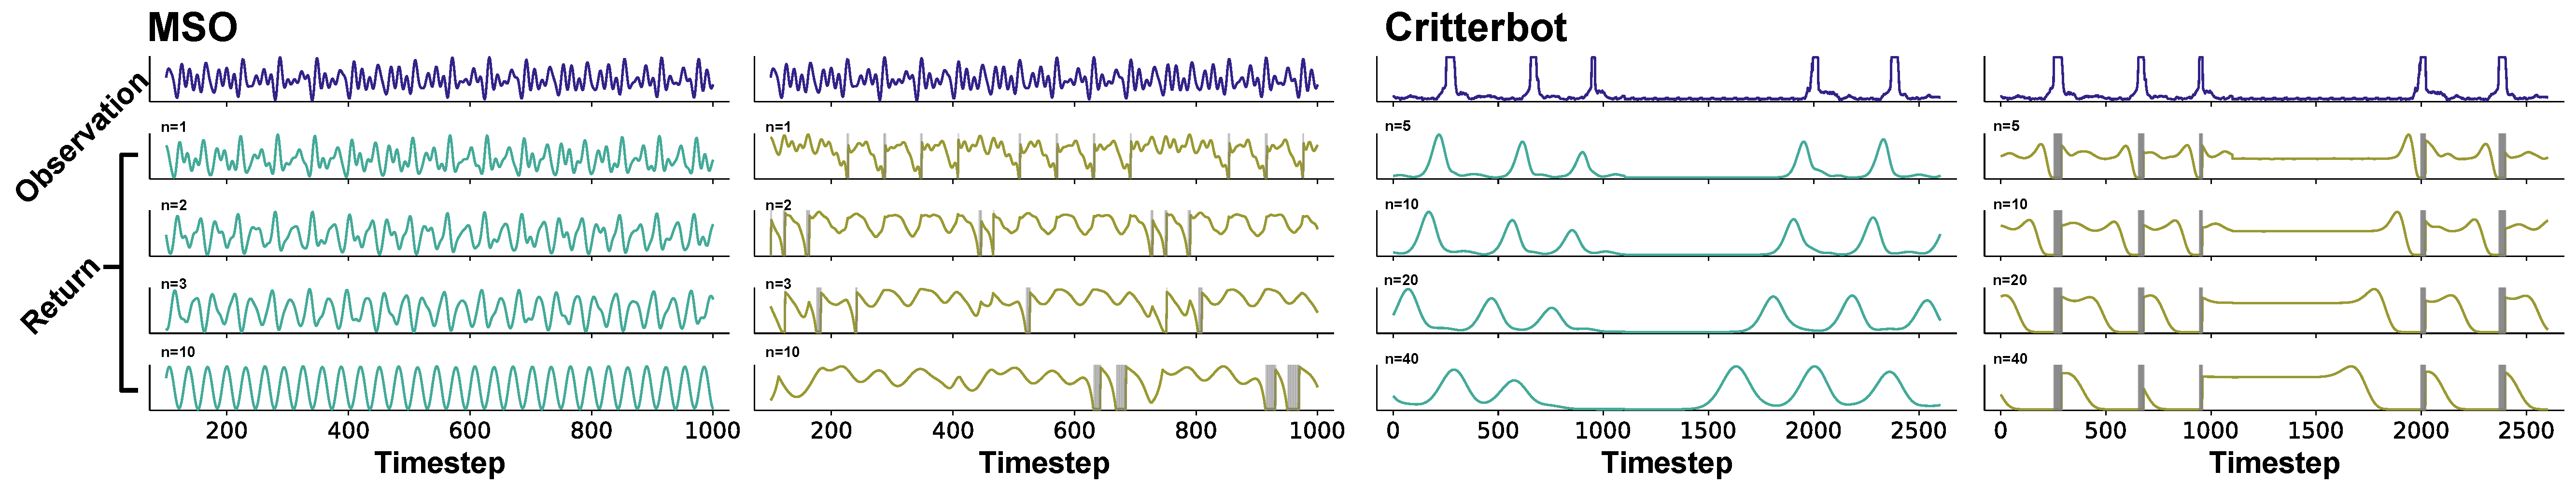
\includegraphics[width=\textwidth]{plots/mso_cb.pdf}
  \caption{(\textbf{left two}) Returns of the multiple sinusoidal
    oscillator (MSO) synthetic data set with constant and terminating
    discount respectively. The gray vertical lines are where the
    return terminates. (\textbf{right two}) Returns of Critterbot
    data set over the light3 sensor with constant and terminating
    discount respectively. \vspace{-0.45cm}}
\end{figure}
%
%

The first series is based off the cycle world, where the agent
observes a sequence of a single active bit followed by $9$ inactive
bits, where the length of the sequence is $m=10$. The cumulant is the observation itself, and in this report we
learn using TD($\lambda=0.9$) with learning rate $\alpha=0.1$ and an underlying tabular representation
where each component is the place in the sequence. We learn two chains
of compositions. The first is that of the continuous discounting
described above, and the second is a series of discounts which
terminate (i.e. $\gamma[t]=0$) when the observation is active.
The predictions of a single run can be seen in figure
\ref{fig:seq_cw}. For the constant discount, as the number of
compositions increases we see the prediction sequence converge to what
looks to be a sinusoid with frequency of $10$, and amplitude driven by
the analysis above. We expect this to be the case following from the
central limit theorem. For the terminating discount, the wave form is
more interesting. The first layer of predictions look very similar to
the constant discount with amplitude shifted by $\frac{\gamma^{m}}{1
  - \gamma^{m}}$. But as there are more compositions the effect seems
to be the prediction is at its height farther away from the active
bit. As the agent gets closer to the observation, the sequence of
summed values is shorter leading to smaller values. Given the sequence
we use it is easy to mistake this as the agent creating a trace of the
cumulant, but we must remember the prediction is about future cumulants.

Next we use a subset of the Critterbot dataset \parencite{modayil2014,
  white2015}, focusing on light sensor 3. This gives a
sequence of spikes similar to the cycle world sequence and a long
pause in-between consistent saturations of the light sensor. We are able to
see with the current setting the predictions look more like
shifted and spread spikes. But with many more compositions, the return
reverts to a similar form as before. The terminating discounts (with
termination at sensor saturation $x[t+1] > 0.99$) provides
a nice demonstration of how the returns are predicting the signal,
just with a decaying prediction instead of the usual growing prediction.
The results are similar in the multiple
sinusoidal oscillator \parencite{jaeger2004harnessing}.
We use a slightly different terminating discount where the return
terminates when the previous normalized prediction is $y^{n-1}[t+1] > 0.9$ rather
than when the observation is saturated. While there are decays as the
MSO sequence peaks, as we increase the depth of the composition, these
periods are less frequent. Deep
compositions may indicate parts of the sequence where there are fewer
saturations in the original sequence.

\section{Future Directions}

% In this paper, we focused on constant discounts and found some
% surprising results. We see compositions as a way to learn complex
% predictions while still taking advantage of the nice properties of
% temporal-difference learning, and the work presented here this is a
% first step in fully appreciating what complex compositions can
% represent.

This work suggests a number of interesting research
directions and questions. While we mostly analyzed the sequence on
discrete steps and applications of the filter, the general form does
lend itself to continuous and complex values of $n$ and $k$. In a similar vein, we
focused on real valued exponential discounting while several
discounting schemes exist which could be applied to our
formulation. We are particularly interested in complex discounting
\parencite{de2018predicting} and hyperbolic discounting
\parencite{fedus2019hyperbolic}. Applying a diverse set of discounting
schemes in compositions provide an interesting way to extend the
power of value functions while maintaining learnability through
efficient algorithms like temporal-difference learning. 



% could lead to more interesting
% predictions which can be learned through efficient algorithms like
% temporal-difference learning.


The approach used in this paper is unable to analyze
state-dependent discount functions. One way around this might be in
analyzing truncated sequences and taking an expectation over a
distribution of sequence lengths. This might lead to a expected
effective discounting sequence, but how this will interact with an
underlying Markov process is unclear. This is an
important next step for understanding the effects of compositions in
general value functions, and could also help in analyzing off-policy
compositions.

Finally, the return can be re-interpreted as a
convolution over the infinite sequence of observations.
While this interpretation
was only used to better the notation in this manuscript, further connections to
convolutions and digital signal processing should be explored.
Better filter designs might inspire different discounting schedules to squeeze more information
from the data stream. We also have only analyzed these convolutions in
the time domain. The frequency domain might give us more insight
into how consistent signals like the cycle world dataset will be
effected by compositions. 



% \begin{itemize}
% \item Discrete, but really the general form is smooth. What does it
%   mean to have partial compositions?
% \item The general formulation gives us a discounting regimen, how
%   does this relate to hyperbolic, other forms of discounting?
% \item Can we analyze state dependent sequences as truncated forms of
%   the time invariant sequence? How would this work?
% \item How does this relate to filters/convolutions in DSP? What other
%   types of functions can we find there?
% \end{itemize}

\vspace{-0.3cm}
\printbibliography

\end{document}

% RLDM requires electronic submissions.  This year's electronic
% submission site is   
% \begin{center}
%    https://cmt3.research.microsoft.com/RLDM2017/
% \end{center}

% Please read the instructions below, and follow them faithfully. Note
% that there is also a template \verb+rldm.rtf+ for Microsoft Word,
% which is available from the website below.


% \subsection{Style}

% Papers to be submitted to RLDM must be prepared according to the
% instructions presented here. Papers consist of a \emph{title}, which
% has a maximum of 100 characters, an \emph{abstract}, which is a
% maximum of 2000 characters, up to five key words, and an
% \emph{extended abstract}, which starts on the second page, and can be
% between one and four pages. Figures and references should be included
% in the latter.

% Authors preferring \LaTeX{} are requested to use the RLDM \LaTeX{}
% style files obtainable at the RLDM website at
% \begin{center}
%    http://www.rldm.org/
% \end{center}
% The file \verb+rldm.pdf+ contains these instructions and illustrates
% the various formatting requirements your RLDM paper must
% satisfy. There is a \LaTeX{} style file called \verb+rldmsubmit.sty+,
% and a \LaTeX{} file \verb+rldm.tex+, which may be used as a ``shell''
% for writing your paper. All you have to do is replace the author,
% title, abstract, keywords, acknowledgements and text of the paper with
% your own. The file
% \verb+rldm.rtf+ is provided as an equivalent shell for Microsoft Word users. 

% \section{General formatting instructions}
% \label{gen_inst}

% The paper size for RLDM is ``US Letter'' (rather than ``A4''). Margins
% are 1.5cm around all sides. Use 11~point type with a vertical spacing
% of 12~points. Palatino is the preferred typeface throughout.
% Paragraphs are separated by 1/2~line space, with no indentation.

% Paper title is 17~point, initial caps/lower case, bold, centered between
% 2~horizontal rules. Top rule is 4~points thick and bottom rule is 1~point
% thick. Allow 0.6cm space above and below title to rules. 

% The lead author's name is to be listed first (left-most), and
% the co-authors' names (if different address) are set to follow. If
% there is only one co-author, list both author and co-author side by side.

% \section{Preparing PostScript or PDF files}

% Please prepare PostScript or PDF files with paper size ``US Letter''.
% The -t letter option on dvips will produce US Letter files.



%%% Local Variables:
%%% mode: latex
%%% TeX-master: t
%%% End:
